\documentclass[tikz,border=6pt]{standalone}
\usepackage{pgfplots}
\pgfplotsset{compat=1.18}
\definecolor{demand}{HTML}{1F4E79}
\definecolor{mr}{HTML}{7EA6C8}
\definecolor{mc}{HTML}{B23A32}
\definecolor{point}{HTML}{C5161D}
\definecolor{areaA}{HTML}{97D4A4}
\definecolor{areaB}{HTML}{E98B73}
\begin{document}
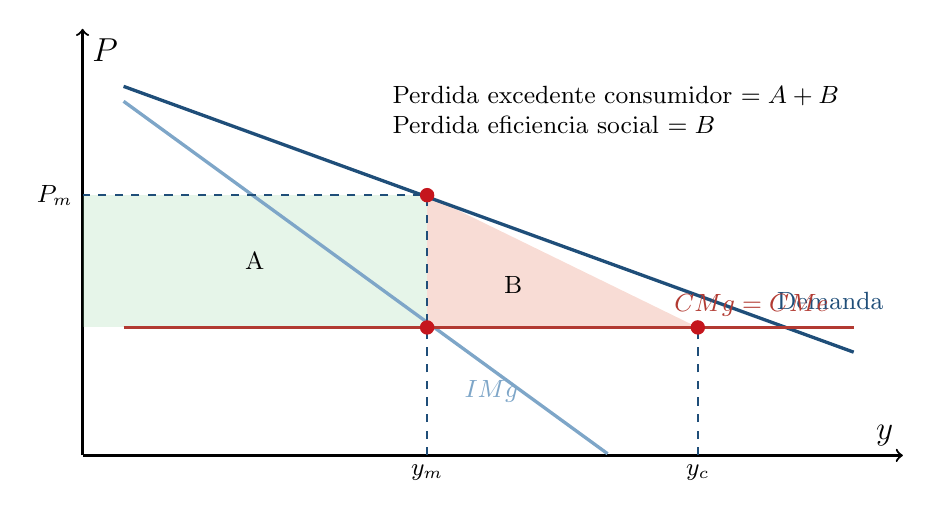
\begin{tikzpicture}
\begin{axis}[width=12cm,height=7cm,axis lines=middle,xmin=0,xmax=10,ymin=0,ymax=10,xtick=\empty,ytick=\empty,xlabel={$y$},ylabel={$P$},axis line style={->,thick},label style={font=\large},tick style={draw=none},clip=false]
\path[fill=areaA,opacity=.24] (axis cs:0,3) rectangle (axis cs:4.2,6.1);
\path[fill=areaB,opacity=.3] (axis cs:4.2,6.1) -- (axis cs:7.5,3) -- (axis cs:4.2,3) -- cycle;
\addplot[domain=.5:9.4,samples=2,very thick,demand] {9-.7*x} node[pos=.88,above right,font=\small] {Demanda};
\addplot[domain=.5:6.4,samples=2,very thick,mr] {9-1.4*x} node[pos=.76,below,font=\small] {$IMg$};
\addplot[domain=.5:9.4,samples=2,very thick,mc] {3} node[pos=.86,above,font=\small] {$CMg=CMe$};
\addplot[dashed,thick,demand] coordinates {(4.2,0) (4.2,6.1) (0,6.1)};
\addplot[dashed,thick,demand] coordinates {(7.5,0) (7.5,3)};
\addplot[only marks,mark=*,mark size=2.4pt,point] coordinates {(4.2,6.1) (4.2,3) (7.5,3)};
\node[left,font=\small] at (axis cs:0,6.1) {$P_m$};
\node[below,font=\small] at (axis cs:4.2,0) {$y_m$};
\node[below,font=\small] at (axis cs:7.5,0) {$y_c$};
\node[font=\small] at (axis cs:2.1,4.55) {A};
\node[font=\small] at (axis cs:5.25,4.0) {B};
\node[align=left,font=\small] at (axis cs:6.5,8.1) {Perdida excedente consumidor $=A+B$\\Perdida eficiencia social $=B$};
\end{axis}
\end{tikzpicture}
\end{document}
